\documentclass[uplatex]{jsarticle}
\usepackage{amsmath}
\usepackage[dvipdfmx]{graphicx}

\setcounter{tocdepth}{3}
\usepackage{float}
\usepackage{moreverb}
\usepackage{lscape}
%\pagestyle{empty}
%\usepackage{wrapfig}
%\usepackage{url}
%\usepackage{EasyLayout}

\usepackage{ascmac}
%\usepackage{fancybx}

%\pagestyle{myheadings}
\usepackage{hyperref}



\begin{document}


\title{二分法とニュートン法の収束の速さについて}
\author{25G1065 塩澤匠生}

%\date{2015年11月13日}
\maketitle


\section{はじめに}
自然界の現象をモデル化するのに方程式が用いられる.
(\ref{eq:omu})式に示されるオームの法則\cite{omu}や(\ref{eq:tou})式に示される等速直線運動\cite{toutyo}については線形の方程式でモデル化できるが
(\ref{eq:dai})式に示されるダイオードの電流電圧特性\cite{daio}や(\ref{eq:jinko})式に示される人口増加\cite{jinko}モデルについては線形であるとモデル化できないため
非線形方程式のまま扱う必要がある.

\begin{equation}
V = IR\label{eq:omu}
\end{equation}
\begin{equation}
x = vt + x_0\label{eq:tou}
\end{equation}
\begin{equation}
I = I_S (e^{\frac{V_D}{n V_T}} - 1)\label{eq:dai}
\end{equation}
\begin{equation}
\frac{dN}{dt} = rN \left(1 - \frac{N}{K}\right)\label{eq:jinko}
\end{equation}


 一般の非線形方程式は解析的に解けないため数値計算に頼る必要がある.
非線形方程式の解を数値計算によって求める手法として中間値の定理によって
解を求める二分法\cite{nibun}と接線を利用して解を求めるニュートン法\cite{nyutonn}というものがある.

 今回はニュートン法と二分法どちらの方が早く解が収束するかを調べる.
調べることでどちらの手法の方が解を早く求められるかが分かる.
解が収束する速さを求める手法としてc言語でのプログラムを用いる.
\section{手法}
% この下の行に入力

\subsection{方程式の説明}

本レポートでは,(\ref{eq:fx})式に示される関数$f(x)$の$f(x)=0$の解を2分法とニュートン法により求める.
この関数を図視すると図\ref{fig:func}のようになる.

\begin{equation}
f(x)=\cos x- x^2\label{eq:fx}
\end{equation}

\begin{figure}[H]
    \centering
    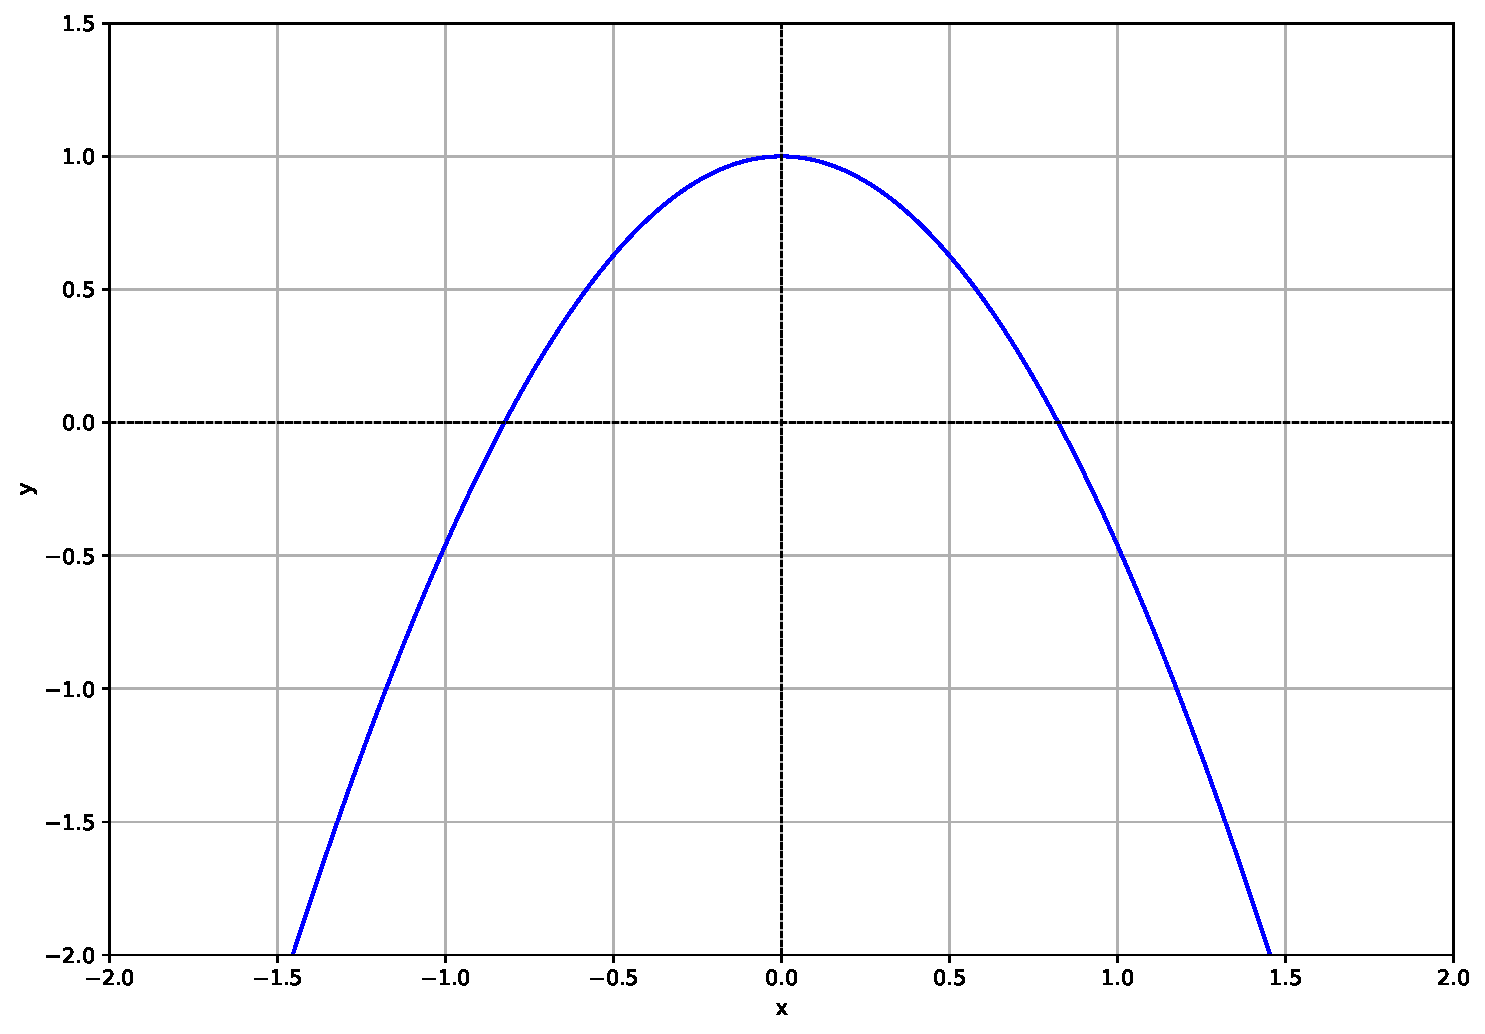
\includegraphics[width=0.9\textwidth]{class_technical_report-main_shiozawaChange/func_graph.pdf}
    \caption{$f(x)=\cos x- x^2$のグラフ}
    \label{fig:func}
\end{figure}


\subsection{2分法・ニュートン法の説明}

まず,二分法についての解説を行う.二分法とは中間値の定理を用いて
方程式の解を求める方法である.中間値の定理とは,関数$y=f(x)$が連続であるとき
x軸上に異なる2点a,b(ただし, a<bとする)
を考えると,f(x)は2点$(a,f(a))$, $(b,f(b))$を通る.
この時,dを$f(a)$と$f(b)$の間の数とすれば,関数は連続であるから,$f(c)=d$
を満たす点cが少なくとも1つaとbの間に存在するというものである.
この中間値を応用し,$f(a)$と$f(b)$が異符号の場合について考る.
まず,区間の中点 $c = (a+b)/2$ を求める.
もし$f(a)$と$f(c)$が異符号、すなわち$f(a)f(c)<0$であれば解は区間$[a,c]$内に存在するため$b$を$c$に更新する.
そうでなければ解は区間$[c,b]$内に存在するため$a$を$c$に更新する.
この操作を反復し、解を含む区間の幅を狭めていくことで解の近似値を得る手法が二分法である.


次にニュートン法についての解説を行う.ニュートン法とは関数$y=f(x)$とx軸との交点を求めるのに接線を利用す
る方法である.まず,特定のx座標$x_0$をきめ,$fd(x_0)=0$となる
$x_0$の接線とx軸の交点のx座標を求め,その座標を$x_{n+1}$として
$x_n$と$x_{n+1}$の差が限りなく0に近づく座標
$x_{n+1}$を$f(x)$の近似解とするものである.
$x_{n+1}$は$x_{n+1} = x_n - \frac{f(x_n)}{f'(x_n)}$
によって求めることができる.



\subsection{プログラムの仕様}

\subsection{評価指標}


\begin{thebibliography}{11}

\bibitem{jikokensuu} NEONAVI, 【自転車事故の実態】を知って安全に利用しよう~令和5年「交通事故統計」から, 
2025年6月11日閲覧,\url{https://neonavi.info/11203/}
\end{thebibliography}
\end{document}



























